%%%%%%%%%%%%%%%%%%%%%%%%%%%%%%%%%%%%%%%%%%%%%%%%%%%%%%%
% ultimate plantUML Cheatsheet
%   by Andreas Offenhaeuser
% Based on MatPlotLib Cheatsheet by Michelle Baltazar https://www.overleaf.com/latex/examples/matplotlib-and-random-cheat-sheet/yttxrcxntbht
%
%%%%%%%%%%%%%%%%%%%%%%%%%%%%%%%%%%%%%%%%%%%%%%%%%%%%%%%

\documentclass{article}
\usepackage[a4paper, landscape, margin=10pt]{geometry}
\usepackage[T1]{fontenc}
\usepackage[dvipsnames]{xcolor}
\usepackage{multicol}
\usepackage{scrextend} % addmargin
\usepackage{tikz}
\usetikzlibrary{decorations.pathmorphing}
\usetikzlibrary{backgrounds}
\usepackage[most]{tcolorbox}

\usepackage{hyperref}
\hypersetup{
    colorlinks, breaklinks,
    linkcolor={red!50!black},
    citecolor={blue!50!black},
    urlcolor={blue!80!black}
}
\parindent0pt
\parskip2pt
\newenvironment{tightcenter}{%
  \setlength\topsep{0pt}
  \setlength\parskip{0pt}
  \begin{center}
}{%
  \end{center}
}
\newcommand{\block}[2]{
  \begin{tikzpicture}[]
  \node [draw=MidnightBlue, fill=white, very thick,
rectangle, rounded corners, inner sep=10pt, inner ysep=10pt] (box){
    \begin{minipage}{0.3\textwidth}
		#2
    \end{minipage}
  };
\node[fill=MidnightBlue, text=white, rounded corners, font=\sffamily, right=10pt] at (box.north west) {\textbf{#1}};
\end{tikzpicture}
}

\newcommand{\code}[1]{
  \begin{tcolorbox}[frame hidden, interior hidden, grow to left by=-5pt,
  boxrule=0pt, boxsep=0pt, arc=0pt, breakable, before skip=4pt, after skip=5pt,]
  \parbox{\textwidth}{\ttfamily\small #1}
  \end{tcolorbox}
}

\newcommand{\header}[3]{
  \title{#1}
  \begin{tikzpicture}[]
  \node [rectangle,anchor=north, minimum width=\textwidth] (title) at (current page.north) {
    \LARGE\textbf{#1}
  };
  \node [anchor=north, outer sep=0] (author) at (title.south) {
    \large #2
  };
  \node [anchor=north east, outer sep=0] (version) at (title.north east) {
    \sffamily\small\color{RubineRed} #3
  };
  \end{tikzpicture}
}

\begin{document}
\vspace{-5pt}
\header{ultimate PlantUML Cheatsheet}{by \href{http://anoff.io}{Andreas Offenhaeuser}}{v.COMMITID}
\vspace{-20pt} % couldn't figure out where the margins come from so force them out
\begin{multicols*}{3}

%%% ICONS %%%
\block{Icons}{
\href{https://useiconic.com/open/}{Open Iconic} is supported out of the box. Any icon can be rendered by embedding into \textbf{<\&..>}.
\code{
card "<\&key> key"

card "<size:42><\&wrench></size>"
}
\begin{tightcenter}
  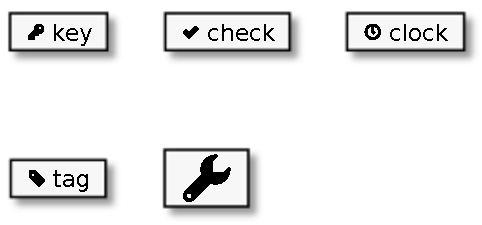
\includegraphics[height=70pt, width=0.45\textwidth, keepaspectratio]{diagrams/dist/icons.pdf}
  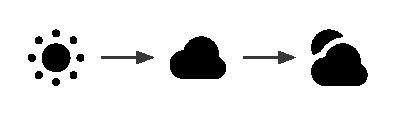
\includegraphics[height=70pt, width=0.45\textwidth, keepaspectratio]{diagrams/dist/icons-transparent.pdf}
\end{tightcenter}

Icons can be shown as icon only by disabling the border and background styles.

\code{
  skinparam cardBorderColor none \\
  skinparam cardBackgroundColor none \\
  skinparam cardShadowing false
}
}

%%% SPRITE ICONS %%%
\block{Sprite Icons}{
Additional icons can be added via sprites. There is a collection of \href{https://github.com/tupadr3/plantuml-icon-font-sprites}{Font Awesome, Developer, Government,.. icons} available via GitHub. Sprites can be included from any location that is reachable by the PlantUML server.

\code{
  !define ICONURL {\scriptsize https://raw.githubusercontent.com/\\
    tupadr3/plantuml-icon-font-sprites/v2.0.0} \\
  !includeurl ICONURL/common.puml \\
  !includeurl ICONURL/font-awesome-5/cogs.puml \\
  !includeurl ICONURL/govicons/submarine.puml \\

  FA5\_COGS(c1, work) \#white \\
  GOV\_SUBMARINE(sub1, Submarine1) \#lightblue \\
  GOV\_SUBMARINE(sub2, , frame, red) \{
  \begin{addmargin}[1em]{0em}
    FA5\_COGS(c2, more work, card, white) \#limegreen
  \end{addmargin}
  \}
}
\begin{tightcenter}
  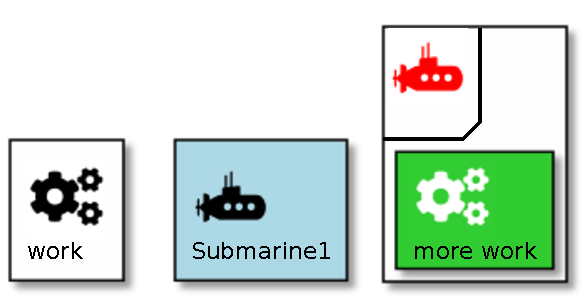
\includegraphics[height=90pt, width=0.9\textwidth, keepaspectratio]{diagrams/dist/icons-sprite.pdf}
\end{tightcenter}
}

%%% COMPONENTS %%%
\block{Components}{
A list of plantUML components and their names, most can be used in any diagrams. The \textit{sequence} diagram only supports a subset.
\begin{tightcenter}
  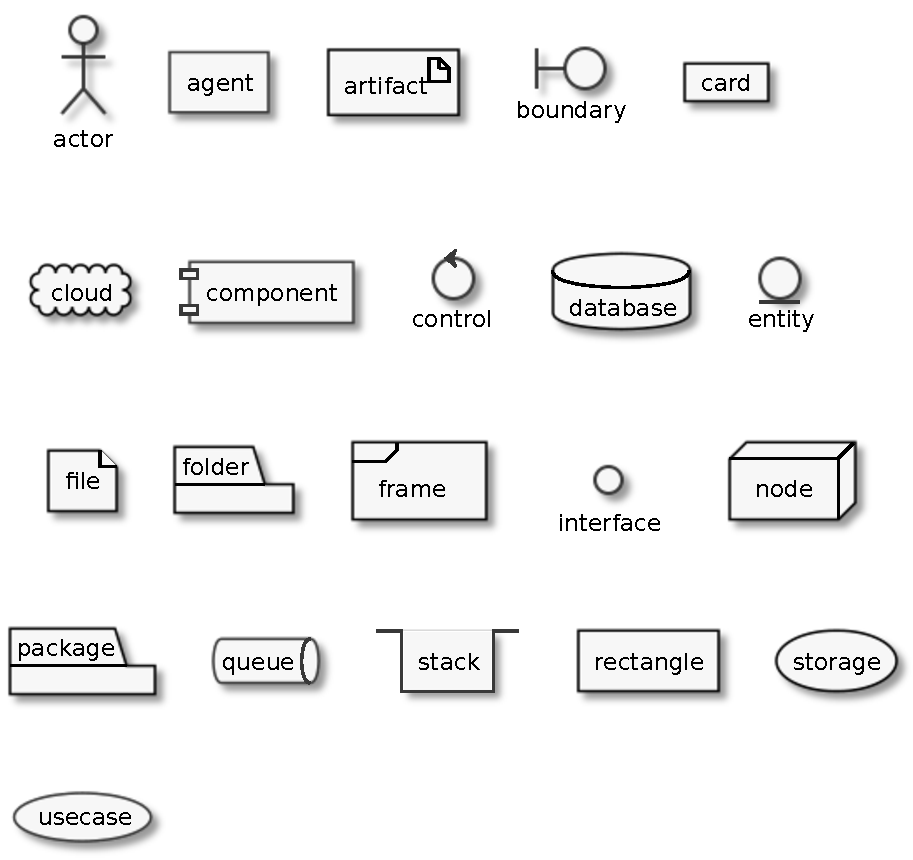
\includegraphics[height=180pt, width=\textwidth, keepaspectratio]{diagrams/dist/components.pdf} 
\end{tightcenter}
}

%%% MULTILINE %%%
\block{Multiline Components}{
Text can be spread across multiple lines in components by declaring the text in \textbf{[ ]}.
\code{
node mynode [
\begin{addmargin}[1em]{0em}
    several \\
    lines \\
    ==== \\
    of \\
    .... \\
    text
\end{addmargin}
]
}
\begin{tightcenter}
  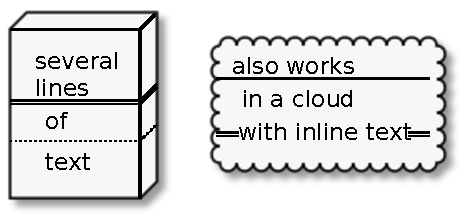
\includegraphics[width=0.7\textwidth]{diagrams/dist/multiline.pdf} 
\end{tightcenter}
}

%%% ARROWS %%%
\block{Arrows}{
All combinations of two arrow heads and line type can be used to create any \href{http://loufranco.com/wp-content/uploads/2012/11/cheatsheet.pdf}{UML arrow type}.

\begin{tightcenter}
  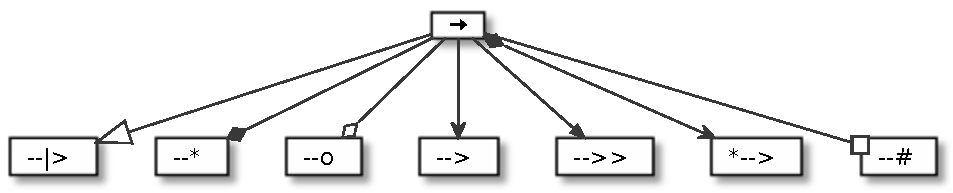
\includegraphics[height=80pt, width=\textwidth, keepaspectratio]{diagrams/dist/arrows.pdf}

  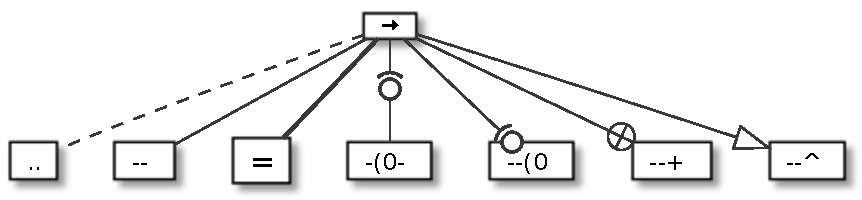
\includegraphics[height=80pt, width=\textwidth, keepaspectratio]{diagrams/dist/arrows-2.pdf}
\end{tightcenter}
}

%%% SKINPARAM %%%
\block{Skinparam Properties}{
For any \textit{component} style properties can be set via
\code{
skinparam <Component><Property> <value>
}

Multiple properties for the same component can be grouped
\code{
skinparam node \{
  \begin{addmargin}[1em]{0em}
  BackgroundColor transparent \\
  BorderColor black
  \end{addmargin}
\}
}

Component properties:

\textit{
  BackgroundColor, 
  BorderColor, 
  BorderThickness, 
  FontColor, 
  FontName, 
  FontSize, 
  FontStyle
}
\newline\newline
Generic properties:

\textit{
  ArrowColor, 
  ArrowLollipopColor, 
  ArrowThickness, 
  BackgroundColor, 
  DefaultTextAlignment {\small ([left], center, right)}, 
  Handwritten {\small [false]}, 
  HyperlinkColor, 
  HyperlinkUnderline, 
  Monochrome {\small [false]}, 
  Nodesep {\small (horizontal margin [0])}, 
  Padding {\small (text padding within node [0])}, 
  Ranksep {\small (vertical margin [0])}, 
  RoundCorner, 
  Shadowing
}
\newline\newline
The full list of \href{http://plantuml.com/skinparam}{skinparam settings} and \href{http://plantuml.com/color}{available colors} can be found on the \href{http://plantuml.com/}{plantUML website}.
}

\end{multicols*}
\end{document}
